\documentclass[]{article} 
\usepackage{pgfplots} 
%\usepgfplotslibrary{external} 
%\tikzexternalize 
\usepgfplotslibrary{fillbetween}
\usepackage{tikz} 
\usepackage{amsmath} 
\usepackage{pgfplots} 
\usetikzlibrary{calc} 
\pgfplotsset{compat = newest, every axis plot post/.style={line join=round}, label style={font=\Large} }
\begin{document} 
	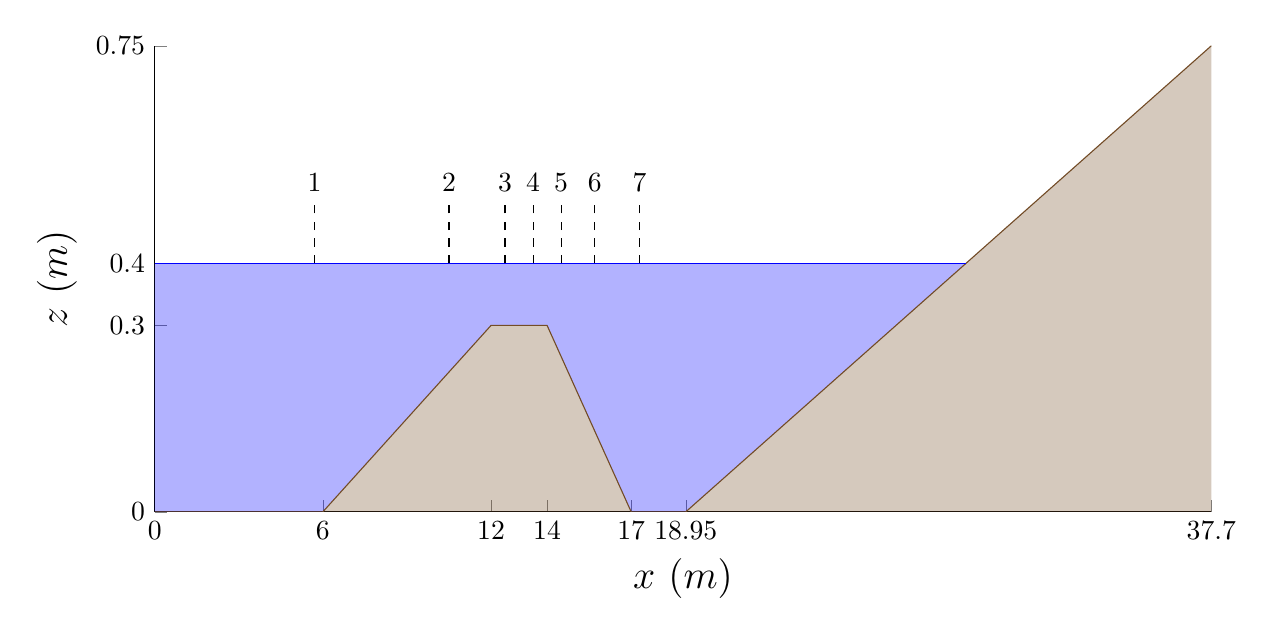
\begin{tikzpicture}
	\begin{axis}[ 
	width = 0.7\textwidth,
	width=15cm,
	height = 7.5cm,
	axis y line*=left,
	axis x line*=bottom, 
	xtick={0,6,12,14,17,18.95,37.7},  
	ytick = {0,0.3,0.4,0.75}, 
	xmin=0, 
	xmax=37.7, 
	ymin =0, 
	ymax = 0.75,
	xlabel=$x$ ($m$), 
	ylabel=$z$ ($m$)]
	
	\addplot [name path=b,brown!60!black] coordinates {(0,0) (6,0) (12,0.3) (14,0.3) (17,0) (18.95,0) (37.7,0.75)};
	
	\path[name path=axis] (axis cs:0,0) -- (axis cs:37.7,0);
	
	\addplot [name path=a,blue] coordinates {(0,0.4) (28.95,0.4)};
	
		\addplot [
		thick,
		color=brown!60!black,
		fill=brown!60!black, 
		fill opacity=0.3
		] fill between[of=b and axis];
		
	\addplot [
	thick,
	color=blue,
	fill=blue, 
	fill opacity=0.3
	] fill between[of=a and b];
	
	
	\addplot [black,dashed] coordinates {(5.7,0.4) (5.7,0.5)};
	\node[above] at (axis cs:5.7,0.5) {1};
	\addplot [black,dashed] coordinates {(10.5,0.4) (10.5,0.5)};
	\node[above] at (axis cs:10.5,0.5) {2};
	\addplot [black,dashed] coordinates {(12.5,0.4) (12.5,0.5)};
	\node[above] at (axis cs:12.5,0.5) {3};	
	\addplot [black,dashed] coordinates {(13.5,0.4) (13.5,0.5)};
	\node[above] at (axis cs:13.5,0.5) {4};
	\addplot [black,dashed] coordinates {(14.5,0.4) (14.5,0.5)};
	\node[above] at (axis cs:14.5,0.5) {5};
	\addplot [black,dashed] coordinates {(15.7,0.4) (15.7,0.5)};
	\node[above] at (axis cs:15.7,0.5) {6};
	\addplot [black,dashed] coordinates {(17.3,0.4) (17.3,0.5)};
	\node[above] at (axis cs:17.3,0.5) {7};
	\end{axis} 
	
	
	
	\end{tikzpicture}
\end{document}